%!TEX root = cscw2018-comic.tex
\subsection{Text Messages Persuade}
Approaches to make a message more attractive and persuasive has long been a focus for a variety of different fields including computational linguistic, social networking, and advertising \cite{smith1996message,tversky1981framing,danescu2012you,huntertowards,maheswaran1990influence,grewal1994moderating}. Among these tactics, message framing is one of the most basic and intuitive methods to generate memorable and persuasive messages \cite{smith1996message,tversky1981framing}. This is mainly because message framing and phrasing generally doesn't require additional information or data visualization. Its simplicity contributes to the various researches on the effect of message framing in memorability. Danescu et.al shows that using unusual word choices and more general theme makes it easier to connect with reader's daily life and makes the message more memorable \cite{danescu2012you}. Using unexpected words and phrases, the message is more likely to capture reader's attention comparing to normal phrases. As for the theme of the message, it should be as general as possible to help readers connect with the message, so it can stay in the reader's mind longer. Beyond the word usage, Tversky and Kahneman found using different reference point to frame the same sentence can result in reader's different response\cite{tversky1992advances,tversky1981framing,kahneman1984choices}.\par
Tversky and Kahneman takes on a unique aspect of the effect of framing. Instead of focusing on the word selection and sentence structure of a quote, Tversky and Kahneman focused on how different reference point of a same sentence can result in reader's different response \cite{tversky1981framing}. It shows that variations of reference point of a decision can determine whether the reader will evaluate it as a gain or a loss, thus changing their decision. For example, choices involving gains are often risk averse and choices involving losses are often risk taking. Meanwhile, implying social norm through the message is another persuasive technique.  Goldstein et. al conducted an interest experiment in the hotel on motivating environmental conservation. They found employing descriptive norms (e.g., "the majority of guests reuse their towels") has more persuasive power than solely mentioning environmental protection. And this normative message gets more persuasiveness when the described setting is closer to individuals' immediate situational circumstances (e.g., "the majority of guests in this room reuse their towels") \cite{goldstein2008room}.  All those techniques are essential for our design of messages to persuade behavioral change.\par


\subsection{Persuade beyond text}
Previous research shows using visual representations are more attractive to readers comparing to text messages \cite{selker2015sweetbuildinggreeter,lin2013impact,scott1993understanding}. Selker et al. retrieves motivational comics from 9GAG, Google, with energy-saving messages, to motivate people's energy saving behaviors and found those comics has higher persuasive power comparing to plain text \cite{selker2015sweetbuildinggreeter}. Persuasive message in a visual form can raise persuadee's awareness and have a greater chance to persuade change. However, this study retrieves the comics from the internet on a certain topic instead of customized generated comic. The drawback of this approach is that it is harder to control the quality and characteristic of the comic. Different authors of comic might have very different drawing style, resulting in differing effects on persuasion.\par
Our work builds on top of the findings of this study that comic can better attract reader's attention. We generate customized comic messages from text messages to unify the comic style and evaluate the persuading effect. Aside from the comparison between text and comics, research has also focused on comparison between other forms of data and their effect in persuading behavioral change. Lin compared two models of presenting information about wind energy in brochure form: (1) photographs and (2) using cartoons as visual aids. To evaluate the effect, the research focused on comparing three measures: (1) audience's knowledge of, (2) attitudes toward, and (3) behavioral intentions regarding wind energy. Results show that there is no significant difference between using photographs or comics in terms of knowledge and attitudes. However, visual aids shown in the cartoon/comics version showed stronger behavioral intentions (e.g., greater willingness to support changes) than the photo group. Because of the abstractness of comics, it can better engage its readers in the messages compared to photographs, making readers more willing to adopt changes. In this study, it mainly focuses on comics' effect on persuading readers to agree on changes conducted by others. However, in our study, we focus on comic's effect on persuading readers themselves to adopt behavior change.\par



\subsection{Communicating through Comics}
Throughout the years, research on evaluating the effect of comic and graphic in communicating ideas have been more and more popular \cite{McDermottPB18,cary2004going,scott1993understanding,weaver2017losing,matsubara2016emotional}. From Scott McCloud's work, it shows that different comic elements have different effects on the ideas and emotion communicated. For example, background shading, character gestures, and word balloon border style can all change the emotion and feeling associated with the message \cite{scott1993understanding,mccloud2011making}. This makes readers more emotionally engaged and more likely to accept the ideas conveyed by the comic. Other comic elements can help engage the readers, for example, research has shown that more abstract comic character can help readers relate themselves with the characters in the comic. This makes readers more engaged to the story and the idea expressed by the comic. Although previous studies have proved that comic can better attract reader's attention and engage them in stories \cite{scott1993understanding,mccloud2011making,McDermottPB18}, the research on using comic to convey formal information and persuade behavioral change is limited.\par
Our study builds on comic's characteristic of attracting reader's attention. We want to further extend the research by understanding if comic can not only engage the readers, but also motivate them to take action. From the study by Haughney, it proposed a comic-style solution to present qualitative research findings. The study proves that the modified comic panel layout for user experience reports can make it more likely for readers to read the whole report through\cite{haughney2008using}. This study offers an innovative idea to present visual information through comic layout. In addition, text bubbles in the layout highlights additional information about the research and can better attract reader's attention compared to text label by the side of a report. However, this design is specifically for presenting visual information such as user interface feedbacks. It is difficult to apply it to other forms of information or research findings. In our study, we utilize comics to present persuasive text posts and extend the research to examine the effect in persuading behavioral change.\par

\subsection{Comics Speak}
\begin{figure}
  \centering
  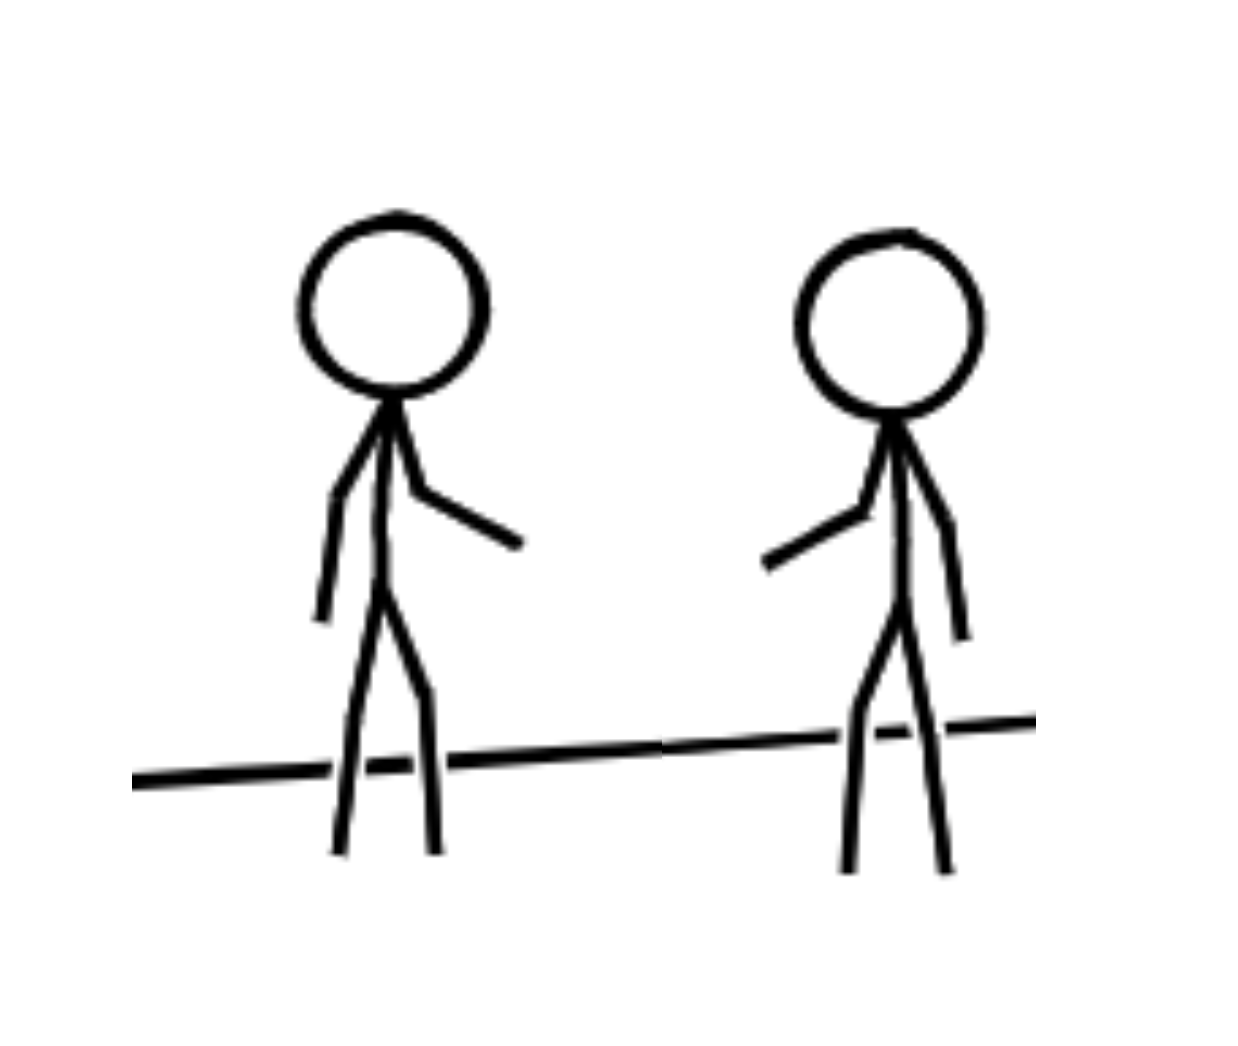
\includegraphics[width=0.3\columnwidth]{figures/xkcd_example}
  \caption{A example of abstract comic figure in XKCD style}
  \label{fig:xkcd}
\end{figure}

As a form of art, the creation of comics has few limitations. Although there is no common template that could describe all comics, if we take a closer look at each comic, it is not hard to see that every comic consists of several fundamental components. We categorize these comic elements into four different groups:
\begin{enumerate}
 \item	characters,
 \item  gesture,
 \item	background shading,
 \item	text bubble,
\end{enumerate}\par
Therefore, to represent a persuasive message in comic form, we need to determine each of those four parameters.\par
As Scott McCloud mentioned in his book, the reader is more likely to project him/herself onto the character in the comic when the comic getting abstract \cite{scott1993understanding}. By taking the perspective of the character, the reader will internalize the information his/her character trying to express or receive. If the information is persuasive, the internalization will imply a higher chance of expected behavior change. Therefore, in this study, we choose to use an abstract yet well-recognized comic style, the xkcd style created by Randall Munroe, in our generated persuasive comic messages \cite{munroe2009xkcd},see Figure~\ref{fig:xkcd}.\par
Beside the abstractness of the character, we believe the relationship between characters is also important. In real world, previous research suggests that messages are more persuasive if the person communicating the ideas is someone the receiver related [citation]. People are more likely to believe their close friends than strangers [citation]. In abstract comics, the relationship between characters is usually modeled by the distance between characters [citation]. So, it is reasonable to believe the link still holds in the world of comics as the reader tends to project his/herself onto the character. Therefore, we hypothesized that the distance between characters in a comic may influence the persuasive power.\par
The gesture of a character is another important component in the comic. The gesture of a character can help reader to understand what happens and the emotion of the character. Different gestures also imply the intensity of an emotion. As a common technique, cartoonists often use the gesture to intensify the feeling that they want to express to the reader. For a persuasive message, the intensified emotion may make the message more memorable than a plain tone. Thus, in this study, the gesture is another key element that we believe may moderate the effectiveness of a comic message.\par
A rich body of research has demonstrated the relationship between color or background shading and the emotion. In comics, the color of elements or the background shading contributes significantly to the feelings as well. However, as xkcd style are mostly seen in black and white, we suspect and confirmed in our pilot study that color backgronud does not go well with generated comics (see pilot test 1). In the main study, we only manipulate the background shading in gray scale to show its affect on the persuasiveness. \par
The word bubble is the most common place in comics to incorporate text information. In a persuasive comic, the word bubble expresses the text content of the message.  \par
